\section{Maximum Margin Classifiers}

\mode<presentation>{
\begin{frame} 
    \begin{center} \huge
        \secname
    \end{center}
    \begin{center}
     What is a \emph{margin} and why should we care about maximizing it?   
    \end{center}
\end{frame}
}

\subsection{Identifying the margin}

\begin{frame}\frametitle{\subsecname}
\mode<article>{
Consider the following linearly separable binary classification problem and the different hyperplanes for separating the two classes. In order to identify the margn of a hyperplane:
}

\only<1-3>{
\begin{enumerate}[(a)]
\item select a hyperplane,
\item select the training point closest to the hyperplane. Call it $\vec x^{*}$. \notesonly{$\vec x^{*}$ has the shortest normal distance to the hyperplane.}
\item measure the normal distance between $\vec x^{*}$ and the hyperplane and call it $\mathrm{d}_{w}$
\end{enumerate}
}
%\begin{figure}[h]
    %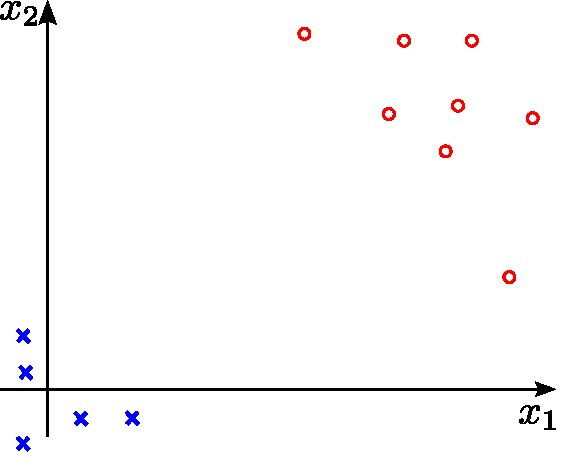
\includegraphics[width=0.5\linewidth]{img/section2_fig13_v2_nomargin_h_none}
    %\mode<article>{
    %\caption{Different hyperplanes for a linearly separable problem.}
    %}
%\end{figure}

\begin{figure}[ht]
     \centering
     \savebox{\imagebox}{
	 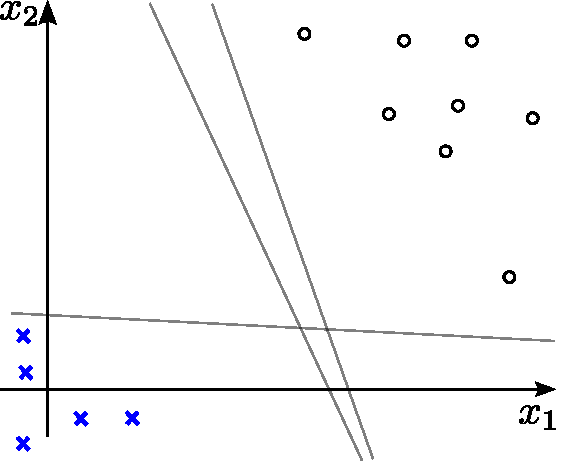
\includegraphics[width=0.35\textwidth]{img/section2_fig13_v2_nomargin_h_multiple}}%
     \only<1>{
     \begin{subfigure}[t]{0.35\textwidth}
         \centering
         \usebox{\imagebox}% Place largest image
         \mode<article>{
         \caption{}
         }
         \label{fig:multiplehyperplanes}
     \end{subfigure}
     }
     \hspace{2mm}
     \only<2>{
     \begin{subfigure}[t]{0.35\textwidth}
         \centering
         \raisebox{\dimexpr.5\ht\imagebox-.5\height}{% Raise smaller image into place
         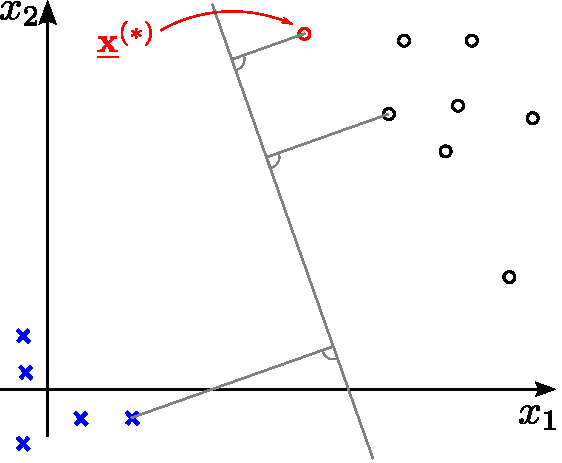
\includegraphics[width=0.99\textwidth]{img/section2_fig13_v2_nomargin_h_closest}
         }
         \mode<article>{
         \caption{}
         }
     \end{subfigure}
     }
     \hspace{2mm}
     \only<3,4>{
     \begin{subfigure}[t]{0.35\textwidth}
         \centering
         \raisebox{\dimexpr.5\ht\imagebox-.5\height}{% Raise smaller image into place
         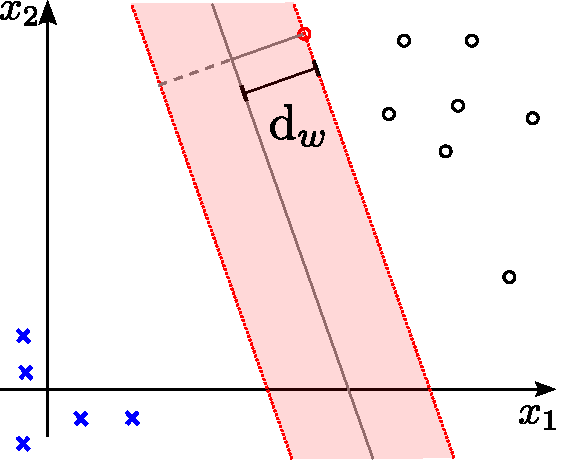
\includegraphics[width=0.99\textwidth]{img/section2_fig13_v2_nomargin_h_margin}
         }
         \mode<article>{
         \caption{}
         }
         \label{fig:margin}
     \end{subfigure}
     \hspace{2mm}
     }
     \only<4>{
     \begin{subfigure}[t]{0.35\textwidth}
         \centering
         \raisebox{\dimexpr.5\ht\imagebox-.5\height}{% Raise smaller image into place
         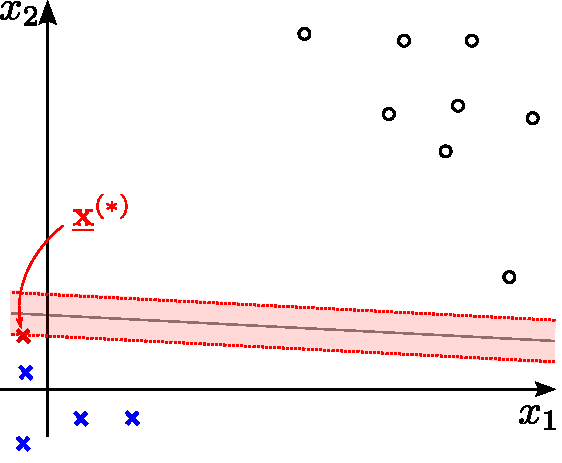
\includegraphics[width=0.99\textwidth]{img/section2_fig13_v2_nomargin_h_marginother}
         }
         \mode<article>{
         \caption{}
         }
         \label{fig:marginother}
     \end{subfigure}
     }
     \mode<article>{
     \caption{Identifying the margin $\mathrm{d}_{w}$ for a hyperplane.}
	 }
	 \label{fig:identifymargin}
\end{figure}
\only<3>{
The distance $\mathrm{d}_{w}$ is the \emph{margin} for that hyperplane.
}
\only<4>{

\question{What are the implications of a wide vs. narrow margin?}

}
    
\end{frame}

\begin{frame}\frametitle{Wide vs. narrow margins}
 
Remember: We are only dealing with a linearly separable problem.


	\begin{figure}[h]
		\centering
		\slidesonly{
		\only<1>{
		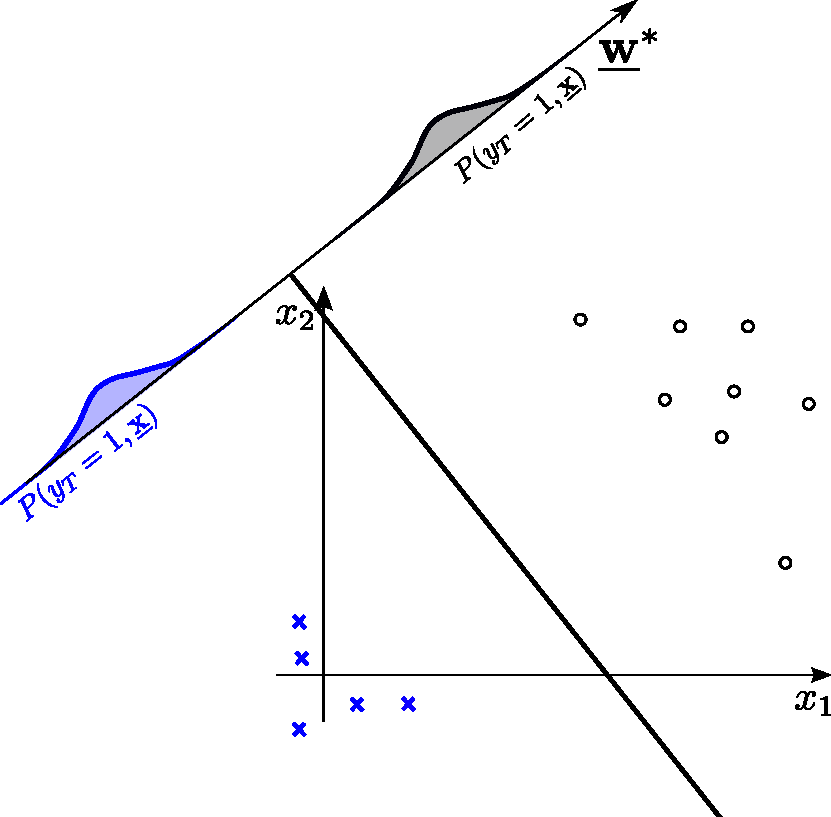
\includegraphics[height=4.5cm]{img/section2_fig13_v2_nomargin_h_distr} 
		}
		}
		\only<2>{
		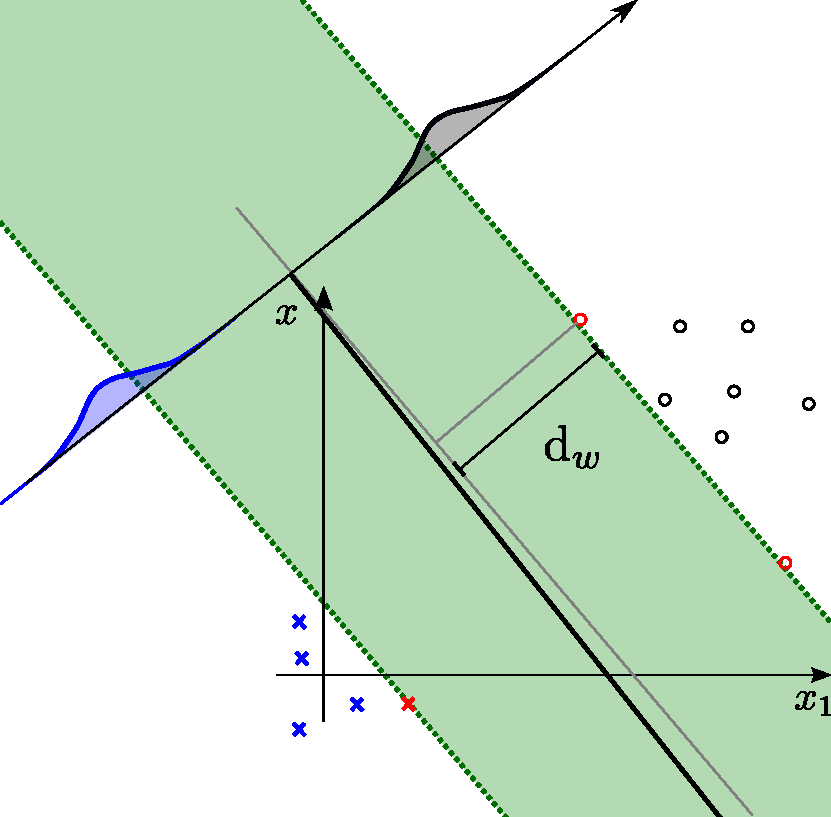
\includegraphics[height=4.5cm]{img/section2_fig13_v2_nomargin_h_margin_max} 
		}
		\mode<article>{
		\caption{
		Potential generalization abilities with maximum margin.
		}
		\label{fig:conditionsv}
		} 
	\end{figure}
 
\mode<article>{
      The {\em margin} is the smallest distance between a separating hyperplane and a training sample. The training sample closest to the decision boundary is denoted with $\vec x^{(*)}$.\\
            Separating the training data with a larger margin is more likely to reduce classification error on unseen data (i.e. lower generalization error, less overfitting).
            A simplistic justification for this: \\
            Assume we have found the separating hyperplane with the maximum margin for perfectly separable data. From this:
            \begin{enumerate}[(1)]
                \item The distance between the classes is at least twice as wide as the distance from the hyperplane to $\vec x^{(*)}$ (i.e. $2 \mathrm{d}_{w}$).
                \item An unseen pattern $\vec x^{(test)}$ is more likely to land closer to training patterns of the same class than patterns from the other class.
                \item The distance between $\vec x^{(test)}$ and $\vec x^{(*)}$ is more likely to be 
                \begin{itemize}
                 \item \emph{larger} than the margin, if the points belong to \emph{different} classes and more likely to be 
                 \item \emph{below} the margin, if both belong to the \emph{same} class.
                 \end{itemize}
            \end{enumerate}
            Another way to look at this:\\
            
            Consider a second hyperplane with the same orientation $\vec w$ but less than maximum (i.e. more narrow) margin. Shift the second hyperplane so that our sample $\vec x^{(*)}$ also lies on the margin of the second hyperplane. The shifting results in the decision boundaries of both hyperplanes appearing parallel to one another, both make contact with $\vec x^{(*)}$. The difference is that the hyperplane with the smaller margin appears to lie inside the first hyperplane. Now consider an unseen pattern $\vec x_{(test)}$ that is very similar to $\vec x^{(*)}$ (i.e. $\vec x_{(test)} = \vec x^{(*)} + \vec {noise}$). $\vec x_{(test)}$ belongs to the same class as $\vec x^{(*)}$. The noise can result in the $\vec x_{(test)}$ falling inside the margin of the first hyperplane. Because the margin of the second hyperplane is more narrow, the decision boundary of that plane is closer to $\vec x^{(*)}$. This means that $\vec x_{(test)}$ is more likely to fall on the wrong side of the second decision boundary and get misclassified (i.e. higher generalization error). This is less likely to happen for the first hyperplane because the maximum margin pushes the decision boundary away from the $\vec x^{(*)}$. We would need to apply more noise on $\vec x_{(test)}$  until it gets misclassified by the maximum margin hyperplane.\vspace{5cm}
            
}
\only<2>{
        \notesonly{Another implication of the maximizing the margin is that}\slidesonly{Also,} the optimal hyperplane with maximum margin is a \emph{unique} solution to the optimization problem.
    }
    
\end{frame}

\subsection{Margins and the VC-dimension}

\begin{frame}

\slidesonly{\vspace{-5mm}} 

\question{Where does the VC dimension come into all of this?}\\

\slidesonly{\vspace{-5mm}} 

\begin{equation}
\, \uparrow \text{margin} \;\; \leadsto \;\; \dvc \, \downarrow   
\end{equation}

\mode<article>{
\begin{figure}[h]
    \centering
    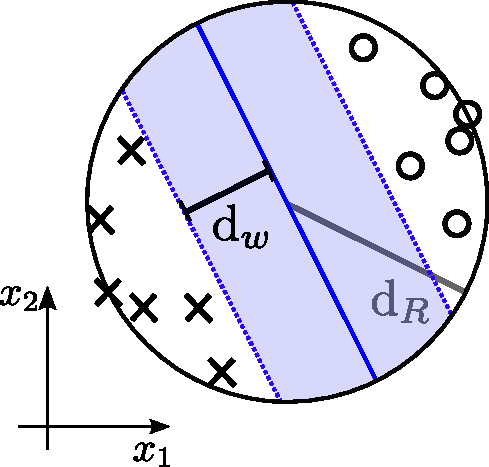
\includegraphics[height=4cm]{img/dvc_margin1} 
    \mode<article>{
    \caption{
    The general setting assumed for deriving the upper bound on the VC-dimension of the maximum margin classifier.
    }
    \label{fig:dvcmarginboundsetting}
    } 
\end{figure}
}
\mode<presentation>{
\placeimage{11.}{6.5}{img/dvc_margin1}{width=3.5cm}
}

\notesonly{        
Large margins imply a small VC dimension. }A larger margin tightens the upper bound of the VC dimension, regardless of the dimensionality of the problem. 

\begin{block}{\textit{Theorem 10.3} in \citep{Vapnik1998}}
\notesonly{states that}

\begin{equation}
    \dvc \quad\leq\quad \min \bigg( \bigg\lfloor 
    \frac{\mathrm{d}_R^2}{\mathrm{d}_{{w}}^2}
\bigg\rfloor, N \bigg) + 1\slidesonly{\qquad\qquad}
\label{eq:dvcmarginbound}
\end{equation}

where,\\

\begin{tabular}{rl}
    $N$\;:& dimension of feature space \\[1mm]
    $\mathrm{d}_w$\;:& the margin: 
        $\frac{1}{\|\vec w \|} \geq \mathrm{d}_w$ \\[1mm]
    $\mathrm{d}_R$\;:& radius of a sphere containing all training points.\\
    &It quantifies the support of $\vec x$:\\
    & $P(\vec x) \neq 0$ for $\|\vec x\| \leq \mathrm{d}_R$ (i.e. no points exist outside of this sphere.)
\end{tabular}
\end{block}

\mode<article>{

The bound in \eqref{eq:dvcmarginbound} assumes a setting as depicted by \figref{fig:dvcmarginboundsetting}. It tells us that, if we draw a sphere around our training data with radius $\mathrm{d}_{R}$ and a second sphere inside of it using the margin $\mathrm{d}_{w}$ as its radius, knowing that the inner sphere is placed in the center and does not contain any datapoints, the theorem then tells us that the VC-dimension is no longer $N+1$ but only as big as the integer component
\footnote{If interested in a proof for \textit{Theorem 10.3}, see 
\href{http://web.eecs.umich.edu/\~jabernet/eecs598course/fall2015/web/notes/lec11\_101315.pdf}
{http://web.eecs.umich.edu/\~jabernet/eecs598course/fall2015/web/notes/lec11\_101315.pdf}
}
\footnote{According to \citep{hush2001vc}, it is debatable whether one should apply $\lfloor \cdot \rfloor$ (floor) or $\lceil \cdot \rceil$ (ceil operation) while pointing out that the latter is possibly incorrect but ``asymptotically sharper'' with reference to \citep{Burges1998}.}
on the ratio $\frac{\mathrm{d}_R^2}{\mathrm{d}_{{w}}^2}$.

}




% illustrations adapted from http://www.cs.columbia.edu/~jebara/4771/notes/class5x.pdf

\mode<article>{
To illustrate:
}

\end{frame}

\begin{frame}\frametitle{\subsecname}

Recall the definition of the $\dvc$ as the \underline{maximal number of training points $p$} that a model can \emph{shatter}.\\

\only<1>{
\begin{figure}[h]
     \centering
     \savebox{\imagebox}{
	 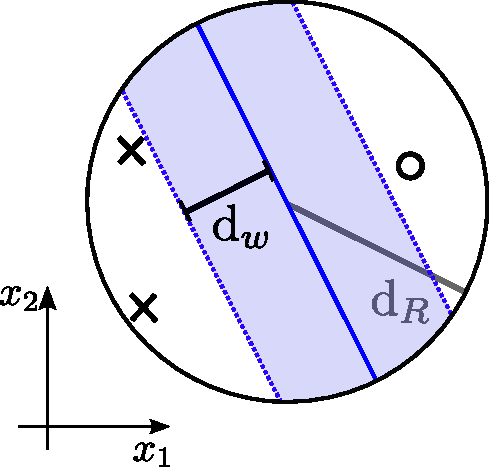
\includegraphics[width=0.22\textwidth]{img/dvc_margin_3pts0}}%
     \begin{subfigure}[t]{0.22\textwidth}
         \centering
         \usebox{\imagebox}% Place largest image
         \mode<article>{
         \caption{}
         }
     \end{subfigure}
     \hspace{2mm}
     \begin{subfigure}[t]{0.22\textwidth}
         \centering
         \raisebox{\dimexpr.5\ht\imagebox-.5\height}{% Raise smaller image into place
         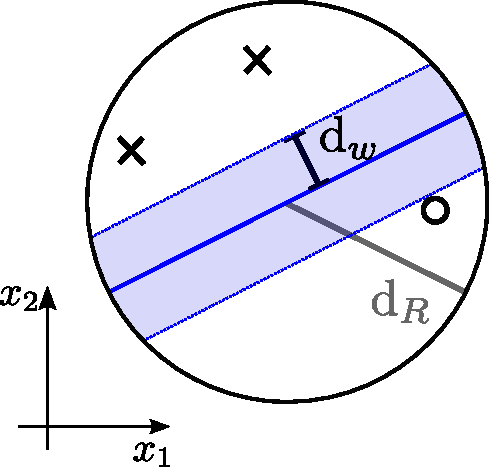
\includegraphics[width=0.99\textwidth]{img/dvc_margin_3pts1}
         }
         \mode<article>{
         \caption{}
         }
     \end{subfigure}
     \hspace{2mm}
     \begin{subfigure}[t]{0.22\textwidth}
         \centering
         \raisebox{\dimexpr.5\ht\imagebox-.5\height}{% Raise smaller image into place
         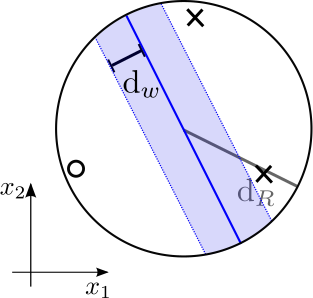
\includegraphics[width=0.99\textwidth]{img/dvc_margin_3pts2}
         }
         \mode<article>{
         \caption{}
         }
     \end{subfigure}
     \mode<article>{
     \caption{A linear neuron can shatter any label configuration of 3 points regardless of how they are arranged in 2D space (excluding colinear points).}
	 }
	 \label{fig:shatter3pts}
\end{figure}

Therefore, $\dvc = N+1 = 3$, for a linear classifier with a margin $0\,\le\,\mathrm{d}_{w}\,<\,\mathrm{d}_{R}$.
}
\only<2>{
As the margin increases, i.e. $\mathrm{d}_{w}\,\rightarrow\,\mathrm{d}_{R}$\notesonly{, $\dvc$ of the linear classifier drops from $N+1$ to $1+1=2$ (e.g. from 3 to 2).}
\slidesonly{
$$
\dvc\;\rightarrow\;2
$$}
In the case of $\mathrm{d}_{w} = \mathrm{d}_{R}$\notesonly{ the VC-dimension will be reducedto 1. But since this implies a dataset of only a single point, it is not such an interesting case.}
\slidesonly{
$$
\dvc\;\rightarrow\;1
$$}


\begin{figure}[h]
     \centering
     \savebox{\imagebox}{
	 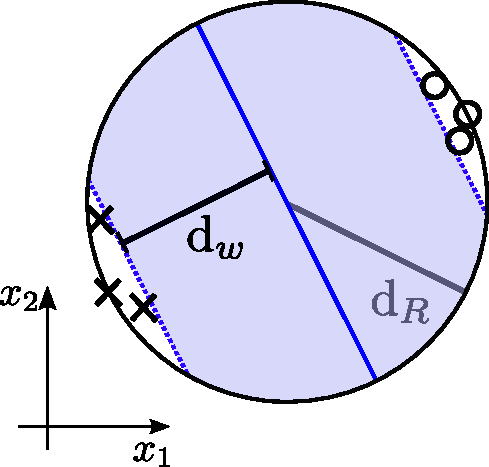
\includegraphics[width=0.22\textwidth]{img/dvc_margin0}}%
     \begin{subfigure}[t]{0.22\textwidth}
         \centering
         \usebox{\imagebox}% Place largest image
         \mode<article>{
         \caption{}
         }
     \end{subfigure}
     \hspace{2mm}
     \begin{subfigure}[t]{0.22\textwidth}
         \centering
         \raisebox{\dimexpr.5\ht\imagebox-.5\height}{% Raise smaller image into place
         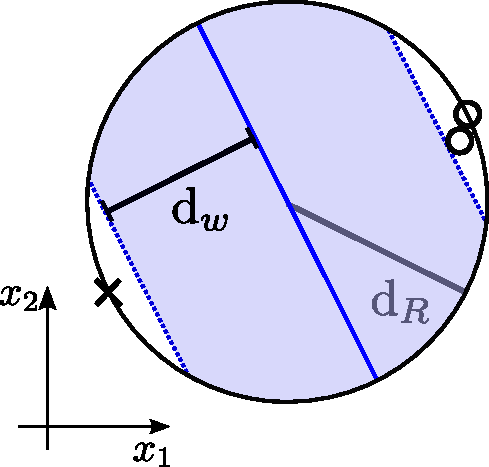
\includegraphics[width=0.99\textwidth]{img/dvc_margin_large}
         }
         \mode<article>{
         \caption{}
         }
     \end{subfigure}
     \hspace{2mm}
     \begin{subfigure}[t]{0.22\textwidth}
         \centering
         \raisebox{\dimexpr.5\ht\imagebox-.5\height}{% Raise smaller image into place
         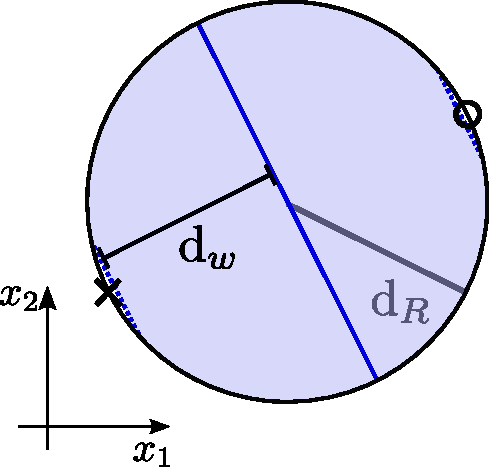
\includegraphics[width=0.99\textwidth]{img/dvc_margin_max}
         }
         \mode<article>{
         \caption{}
         }
     \end{subfigure}
     \mode<article>{
     \caption{A linear neuron can no longer shatter $N+1$ points when the margin is maximal.}
	 }
	 \label{fig:shatter3pts}
\end{figure}
}
     
            
            
\end{frame}

\begin{frame}
\only<1,4>{
If the margin provides a bound for the $\dvc$
}
\only<1,4>{
\mode<presentation>{ 
$$
    \dvc \quad\leq\quad \min \bigg( \bigg\lfloor 
    \frac{\mathrm{d}_R^2}{\mathrm{d}_{{w}}^2}
\bigg\rfloor, N \bigg) + 1\slidesonly{\qquad\qquad}
$$
}
}
\only<1->{

\question{What were the benefits of reducing $\dvc$?}

%leave line break for effective pause
}
\only<2,3>{
Recall\notesonly{ that one of the key results of Statistical Learning Theory was the formulation of the bound on the generalization error, given a finite set of samples:}
\notesonly{
\begin{equation}
    P \bigg\{ \sup_{\vec{w} \in \Lambda} \Big| R_{[\vec w]} 
        - R_{\emp [\vec{w}]}^{(p)} \Big| > \eta \bigg\} 
    < 4 \exp \Big( G_{(2p)}^\Lambda - p 
        \big( \eta - \smallfrac{1}{p} \big)^2 \Big)
    \eqexcl \epsilon
\end{equation}

where $\Lambda$ denotes the model class and $G^{\Lambda}_{(2p)}$ denotes the growth function\footnote{cf. lecture 2.1.3 on Statistical Learning Theory and corresponding notes.}.
}

With a probability larger than $\,1 - \epsilon\,$ we obtain:

\begin{equation}
    R_{[\vec w]} < \underbrace{R_{\emp [\vec{w}]}^{(p)}
        }_{\substack{\text{empirical}\\\text{error}}} +
        \underbrace{\bigg(
        \smallfrac{G_{(2p)}^\Lambda - \ln \frac{\epsilon}{4}}{p}
        \bigg)^{\frac{1}{2}} \,+\, \frac{1}{p}
        }_{\text{complexity term}~C(p,\dvc)}
        \label{eq:generalizationresultsriskgrowth}
\end{equation}

\notesonly{For a given $\epsilon$, the complexity term
only depends on $p$ and $\dvc$.}}
\mode<article>{
 Therefore, the VC dimensions helps in formulating a bound on the \textbf{generalization ability} of Empirical Risk Minimization (ERM). 
 Knowing that 
 }
 \only<2,3>{
 \begin{itemize}
  \notesonly{\item the risk $R_{[\vec w]}$ and empirical risk $R_{\text{emp}[\vec w]}$ are represented by the generalization $E^{G}_{[\vec w]}$ and training error $E^{T}_{[\vec w]}$, respectively:\\
  $R_{[\vec w]} \, \corresponds \, E^{G}_{[\vec w]}\,,$
  $
  R_{\text{emp}[\vec w]}  \, \corresponds \, E^{T}_{[\vec w]}
  $
  and that} 
  \item for $p>\dvc$:
  $$G^{\Lambda}_{(p)} \le \dvc \Big(\ln \frac{p}{\dvc} + 1\Big)\,,$$
  \end{itemize}
  }~\notesonly{
\eqref{eq:generalizationresultsriskgrowth} can be reformulated in order to  highlight the relationship between the VC dimension and the generalization ability of the model class:}\\

\notesonly{For a finite training set, the generalization error is bound with probability $1-\epsilon$:}
\only<4,5>{
\slidesonly{\vspace{-7mm}}
\begin{equation}
    E^{G}_{[\vec w]} \;\le\; E^{T}_{[\vec w]} + 
    \underbrace{
    \sqrt{\frac{\dvc \left(\ln \frac{2\,p}{\dvc} + 1\right)-\ln\frac{\epsilon}{4}}{p}}}_{\text{generalization gap}} + \frac{1}{p} \quad \text{for } p > \dvc
    \label{eq:generalizationresults}
\end{equation}

\question{What about $\dvc \rightarrow 0$? Is this ideal?}

%\begin{equation}
%\boxed{
%\;
%\uparrow \, \text{margin}
%\quad \leadsto \quad
%\dvc \, \downarrow 
%\;   
%}
%\end{equation}  
}

\only<5>{
\begin{figure}[h]
    \centering
    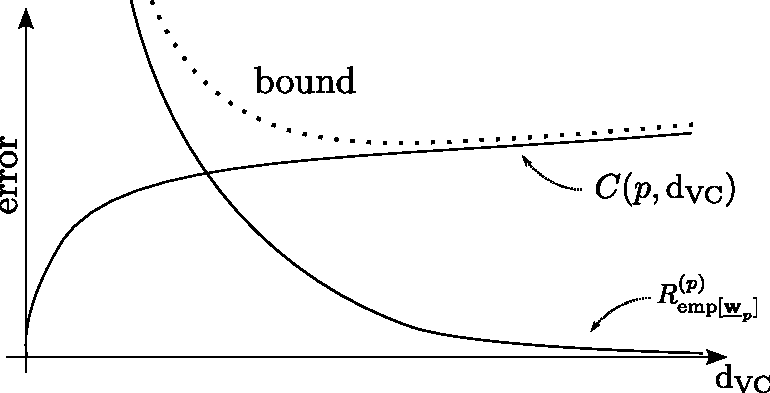
\includegraphics[height=3.5cm]{img/section2_fig12_v2} 
    \mode<article>{
    \caption{
    The effect of the VC-dimension and bias-variance trade-off
    }
    \label{fig:dvcbiasvariance}
    } 
\end{figure}

}

\end{frame}


